\documentclass[10pt]{article}

% The following command leaves more space between lines.  That's great
% when correcting drafts.  When you comment it out, however, the
% output looks much nicer.
%
\linespread{1.0}

\usepackage{amsmath}
\usepackage{amssymb}
\usepackage{graphicx}
\usepackage{epsfig}
\usepackage{latexsym}
\usepackage{amsthm}

\usepackage{mathrsfs}

\usepackage{multicol}



\usepackage[colorlinks,citecolor=blue]{hyperref}

\usepackage[latin1]{inputenc}

\usepackage{tikz-cd}
\usepackage{pgfplots}

%\usepackage{3dplot}

\usetikzlibrary{matrix,arrows,decorations.pathmorphing}


\usepackage[scale=0.8]{geometry}


%\usepackage{umoline}\setlength{\UnderlineDepth}{1pt}
%\usepackage[linktocpage=true]{hyperref}

\input xy
\xyoption{all}


%\addtolength{\hoffset}{-.5in}
%\addtolength{\textwidth}{1in}
%\setlength{\parindent}{.5in}
%\setlength{\textheight}{9.5in} \setlength{\topmargin}{-2cm}


\pagestyle{myheadings}\parindent 0em




\usepackage[latin1]{inputenc}


%------------------copy and posted code from the internets-------------

%\numberwithin{equation}{section} % comment out when neccessary

\newtheorem{theorem}[equation]{Theorem}
\newtheorem{lemma}[equation]{Lemma}
\newtheorem{proposition}[equation]{Proposition}
\newtheorem{corollary}[equation]{Corollary}


\theoremstyle{definition}
\newtheorem{definition}[equation]{Definition}
\newtheorem{example}[equation]{Example}
\newtheorem{remark}[equation]{Remark}
\newtheorem{problem}[equation]{Problem}



\newcommand{\R}[1]{\mathbb{R}^{#1}}
\newcommand{\C}[1]{\mathbb{C}^{#1}}
\newcommand{\Z}[1]{\mathbb{Z}^{#1}}
\newcommand{\K}[1]{\mathbb{K}^{#1}}
\newcommand{\embed}[0]{\hookrightarrow}
\newcommand{\TT}[4]{\begin{tabular}{| c | c |}\hline $#1$ & $#2$ \\ \hline $#3$ & $#4$ \\ \hline\end{tabular}} %goddamn it
\newcommand{\partd}[2]{\frac{\partial #1}{\partial #2}}
\newcommand{\limit}[2]{\displaystyle{ \lim_{#1 \to #2}}}
\newcommand{\vectornorm}[1]{\left|\left|#1\right|\right|}
\newcommand{\Ker}[0]{\text{\textnormal{Ker}}}
\newcommand{\Hom}[0]{\text{\textnormal{Hom}}}
\newcommand{\circled}[1]{\tikz[baseline=(char.base)]{
            \node[shape=circle,draw,inner sep=2pt] (char) {#1};}}


\newcommand{\T}{\rotatebox[origin=c]{180}{$\scriptscriptstyle \perp $}}
\newcommand{\x}{\textbf{x}}
\newcommand{\y}{\textbf{y}}
\newcommand{\supp}{\text{\textnormal{supp}}}
\newcommand{\csupp}{\text{\textnormal{cosupp}}}
\newcommand{\found}{\text{\textnormal{found}}}
\newcommand{\roof}{\text{\textnormal{roof}}}

\newcommand{\bcup}{\displaystyle\bigcup}
\newcommand{\bcap}{\displaystyle\bigcap}
\newcommand{\dsum}{\displaystyle\sum}
\newcommand{\dint}{\displaystyle\int}





\begin{document}
%

{\bf Name:} \hrulefill\hrulefill\hrulefill\\
{\bf M143} \qquad \qquad \\
{\bf Limits and Continuity}\\ %(look familiar??)\\
%Show all work for full/partial credit.
%---------------- End of the document ---------------

\section{Limits}

Informally, the limit of a function $\limit{x}{a} f(x)=L$ (if it exists) is a number $L$ such that when $f(x)$ get's closer and closer to $a$, $f(x)$ gets closer and closer to $L$. \\

Consider the function $f(x)=\frac{x^2-1}{x-1}$, what happens as $x$ get's closer and closer to 1?

$$
\begin{array}{|c|c|}
\hline
x & f(x)\\
\hline
1.1 & 2.1\\
1.01 & 2.01\\
1.001 & 2.001\\
.9 & 1.9\\
.99&1.99\\
.999 & 1.999\\
\hline
\end{array}$$

You can test and see these values here: \url{https://www.desmos.com/calculator/w3ycpf3mv4}.  It certainly seems as if $x$ gets closer and closer to $1$, $f(x)$ approaches the value $2$.  Why couldn't we just plug in 1?  Because if we did we would get $f(1)``="\frac{1^2-1}{1-1}``="\frac{0}{0}$ which is undefined.  Recall that $1$ would not be a part of the domain of $f(x)$.  This, in fact, is the whole point of limits, the entire reason they exist, is in order to give values to things like $f(1)$ which are not defined.\\

The left and right limits of a function are values the function approaches as $x$ $a$ from the left or the right, so as we see above, they both (the black and orange dots in the linked graph) both approach the same value.  So:

\begin{itemize}
\item $\limit{x}{1^-}\frac{x^2-1}{x-1}=2$.
\item $\limit{x}{1^+}\frac{x^2-1}{x-1}=2$
\item $\limit{x}{1}\frac{x^2-1}{x-1}=2$
\item $f(1)$ is undefined.
\end{itemize}

So looking at this graph:
$$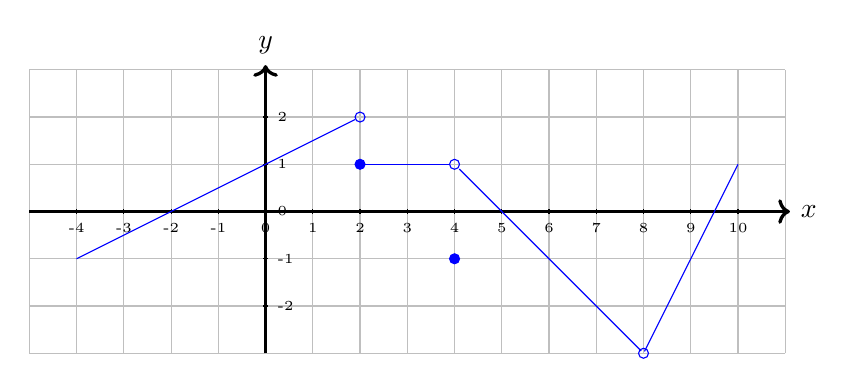
\begin{tikzpicture}[scale=.6][domain=-5:11]
    \draw[gray!50, thin, step=1] (-5,-3) grid (11,3);
    \draw[very thick,->] (-5,0) -- (11.1,0) node[right] {$x$};
    \draw[very thick,->] (0,-3) -- (0,3.1) node[above] {$y$};

    \foreach \x in {-4,...,10} \draw (\x,0.05) -- (\x,-0.05) node[below] {\tiny\x};
    \foreach \y in {-2,...,2} \draw (-0.05,\y) -- (0.05,\y) node[right] {\tiny\y};

    \draw[blue] (2,2) circle (3pt);
    \draw[ blue, fill] (2,1) circle (3pt);
    \draw[blue] (4,1) circle (3pt);
    \draw[fill, blue] (4,-1) circle (3pt);
    \draw[blue] (8,-3) circle (3pt);


  \draw[scale=1,domain=-4:1.9,smooth,variable=\x,blue] plot ({\x},{.5*\x+1});
  \draw[scale=1,domain=2.1:3.9,smooth,variable=\x,blue] plot ({\x},{1});
  \draw[scale=1,domain=4.1:7.95,smooth,variable=\x,blue] plot ({\x},{-1*\x+5});
  \draw[scale=1,domain=8.02:10,smooth,variable=\x,blue] plot ({\x},{2*\x-19});


\end{tikzpicture}$$

For $x=2,4,6,8$, find the left and right limits, the limit, and the value of the function.  See if you understand why the following are true:

\begin{itemize}
\item $\limit{x}{2^-}f(x)=2$, as we approach $x$ from the left, this is what $f(x)$ approaches.
\item $\limit{x}{2^+}f(x)=1$, as we approach $x$ from the right, this is what $f(x)$ approaches.
\item $\limit{x}{2}f(x)$ is undefined, there is no single number that $f(x)$ get's closer to, so there is no limit.
\item $f(2)=1$, that's the actual value of $f(2)$.
\end{itemize}

Similarly, we should see:

\begin{itemize}
\item $\limit{x}{4^-}f(x)=1$.
\item $\limit{x}{4^+}f(x)=1$.
\item $\limit{x}{4}f(x)=1$.
\item $f(4)=-1$.
\item $\limit{x}{6^-}f(x)=-1$.
\item $\limit{x}{6^+}f(x)=-1$.
\item $\limit{x}{6}f(x)=-1$.
\item $f(6)=-1$.
\item $\limit{x}{8^-}f(x)=-3$.
\item $\limit{x}{8^+}f(x)=-3$.
\item $\limit{x}{8}f(x)=-3$.
\item $f(8)$ is undefined.
\end{itemize}

A great shorthand for determining when there is or isn't a limit is: ``$\limit{x}{a}f(x)=L$ and exists if and only if $\limit{x}{a^-}f(x)=L$ and $\limit{x}{a^+}f(x)=L$"

\section{Continuity}

I'm not going to overblow continuity with to much verbiage here since we intuitive understand what it means to be continuous, it just means that all the points ``connect".  So what does tat mean for us above?  Out of the values $x=2,4,6,8$, where is $x$ continuous?

It seems like it's only 6 where it's continuous.  2 and 4 have jump discontinuities, and $f(x)$ isn't even defined at $x=8$ so how could it be continuous there?  So the definition of continuous is as intuitive as we would like:\\

$f(x)$ is continuous at $a$ if and only of $f(a)=\limit{x}{a} f(x)$.  So as in above, out of the 4 points we looked at, $x=6$ is the only place where everything ``behaves properly" and we get continuity.


























\end{document}
